\section{Einleitung}

Diese Dokumentation gibt einen Überblick über das Semesterprojekt im Modul Software-Engineering des Masterstudienganges Medieninformatik.
Ziel des Projekts ist es, eine anwendungsspezifische Sprache (domain-specific language)\todo{DSL einführen} zu entwickeln und anhand dieser Code einer höheren Programmiersprache zu generieren.
Der generierte Code soll hierbei eine zu implementierende Anwendung komplettieren und somit der Umgang mit anwendungsspezifischen Sprachen sowie der Codegenerierung praxisnah geübt und gefestigt werden.

Die Anforderung wird anhand eines Spiels und eines Levelgenerators umgesetzt.
Der Levelgenerator übernimmt hierbei die Verarbeitung der anwendungsspezifischen Sprache.

\subsection{Spielidee}

Es soll ein 2D Spiel in Top-Down Perspektive entwickelt werden.
Das Spielziel ist es, ein sich ständig leerendes Bier rechtzeitig durch den Besuch eines \textit{Spätis}\footnote{Späti ist eine, in Berlin gebräuchliche, Abkürzung für Spätverkaufsstelle. Spätis verkaufen, mitunter die ganze Nacht über, unter anderem Bier und sind somit die ``Tankstelle'' der trinkenden Nachtschwärmer.}
wieder aufzufüllen und bis zum Ende einer vorher definierten Zeit das Bier nicht leer werden zu lassen.
Dazu bewegt der Spieler sich in einer blockbasierten Welt.
Diese enthält sowohl Spätis zum nachfüllen des Bieres, als auch Gegner welche den Füllstand des Bieres oder die Geschwindigkeit des Spielers reduzieren können.
Gegner besitzen eine gewisse Intelligenz und können den Spieler verfolgen sobald sie ihn gesehen haben.
Abbildung \ref{fig:einleitung:screenshot} zeigt eine typische Szene des Spiels.
Die Statusbalken am unteren Bildrand geben Auskunft über den aktuellen Füllstand des Bieres (links), sowie die verbleibende Zeit (rechts) welche der Spieler überbrücken muss um das Level erfolgreich abzuschließen.

\begin{figure}[]
\centering
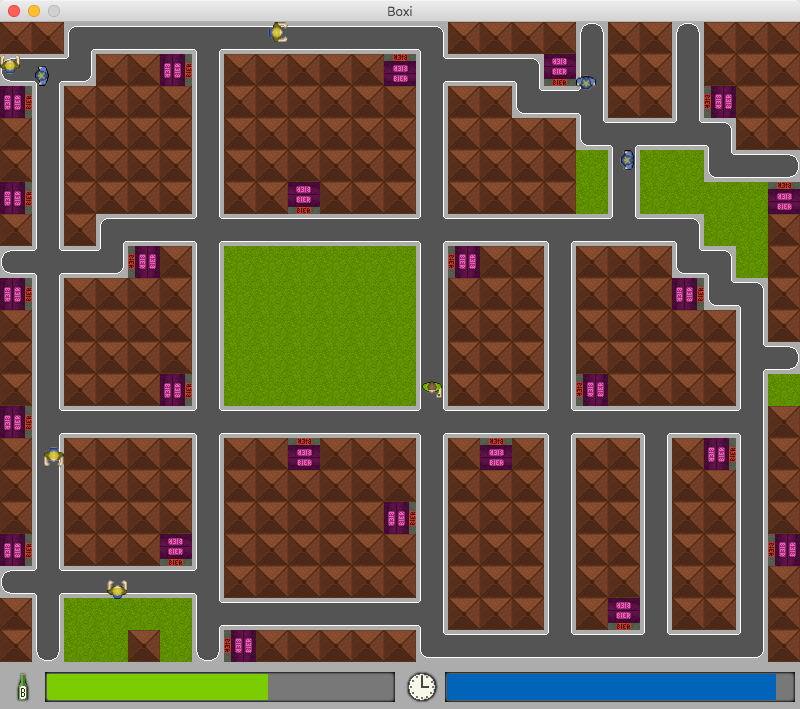
\includegraphics[width=3in]{img/02_screenshot.png}
\caption{Screenshot des Spiels}
\label{fig:einleitung:screenshot}
\end{figure}


\subsection{Zweck der Codegenerierung}

Das Spiel beinhaltet mehrere Level.
Ein Level beinhaltet beispielsweise Informationen über die Anordnung der Blöcke auf der Karte oder die Lauf- und Trinkgeschwindigkeit des Spielers.
Dazu wurde eine anwendungsspezifische Sprache und ein Codegenerator entwickelt, auf welchen in Abschnitt \ref{sec:levelerzeugung} näher eingegangen wird.